\documentclass[sigplan,10pt,review,anonymous,balance=false,pbalance=false]{acmart}
\pdfmapfile{+libertine.map}
\pdfmapfile{+zi4.map}
\pdfmapfile{+newtx.map}
\pdfmapfile{+lm.map}
\pdfmapfile{+cm.map}
\pdfmapfile{+amsfonts.map}
\settopmatter{printacmref=false}
\setcopyright{none}
% Omit speculative conference date/location metadata in anonymous review draft.
\acmConference[CC 2027]{International Conference on Compiler Construction}{2027}{}
\acmYear{2027}
\acmISBN{}
\acmDOI{}
\usepackage{amsmath,booktabs,graphicx,xurl,microtype,listings}
\raggedbottom
\emergencystretch=2em
\newcommand{\ps}{\mathbin{\psi}}
\newcommand{\rav}{\operatorname{rav}}
\newcommand{\red}{\operatorname{red}}
\title{Mechanizing Mathematics of Arrays: From \texorpdfstring{$\psi$}{Psi} Reduction to Machine-Shaped Attention Kernels}
\begin{document}
\begin{abstract}
We mechanize attention in the Mathematics of Arrays (MoA), starting from a typed $\psi$-indexed denotational normal form (DNF). The compiler derives $\gamma$ addresses and an $\Omega$-lifted operational normal form for a selected machine shape. Replay reproduces four archived compiler ASTs and byte-identical OpenMP C. We compare hand and compiler score and value selections under bound-index renaming and validate generated executions independently. On an NVIDIA A100-SXM4-80GB, the generated OpenACC realization returns both the attention weights and output in FP64. Across 224 timed calls at eight held-out sizes and four candidate shapes, the largest recorded absolute errors were $2.78\times10^{-17}$ and $2.26\times10^{-16}$, respectively. Predicted time met the 25\% error threshold at six sizes. At $N=64$ and $128$, errors were 57.75\% and 28.88\%. The frozen model chose $\Omega\langle256\rangle$ throughout, matching the lowest observed median at seven sizes and within 5\% at all eight. The fixed $\langle256\rangle$ rule yields identical selections. A completed companion correspondence study covers 44 paired implementations across Papers I--IV: 246 end-DNF component comparisons and matching operational C structures, with lifted equality under common admissible machine contracts. All 138 untimed pair checks give zero difference. These results establish implementation correspondence; they add no new hardware timings. We also identify the remaining validation boundary for the ten-field model.
\end{abstract}
\begin{CCSXML}
<ccs2012>
 <concept><concept_id>10011007.10011006.10011008</concept_id><concept_desc>Software and its engineering~General programming languages</concept_desc><concept_significance>300</concept_significance></concept>
</ccs2012>
\end{CCSXML}
\ccsdesc[300]{Software and its engineering~General programming languages}
\keywords{Mathematics of Arrays, compiler correctness, denotational normal form, operational normal form, machine shape, forward attention}
\maketitle
\thispagestyle{plain}
\pagestyle{plain}
\section{Introduction}
The original Paper~I forward-attention kernels were derived by hand using the Mathematics of Arrays (MoA)~\cite{paperI,moa}. In MoA, $\rho$ specifies shapes, $\langle i\rangle\psi A$ selects components, $\iota(\rho A)$ enumerates legal indices, and $\tau(A)=\prod(\rho A)$ counts components. The derivation reduces indexed expressions to a denotational normal form (DNF), derives addresses with a layout $\gamma$, and lifts execution with $\Omega$ to a target machine array. We ask which steps a compiler can perform and which properties an independent checker can verify.

Paper I forward attention~\cite{paperI} supplies the worked trace and physical baseline; the completed companion correspondence inventory extends the semantic and operational checks across Papers I--IV. The original hand-derived implementations and ACCESS measurements establish the historical baseline; they were \emph{not} compiler outputs. We ask the compiler to preserve the same selected-component semantics, expose its intermediate ASTs, derive addressed and lifted representations, and emit an executable realization. Different reduction sequences are acceptable, but their canonical DNFs must agree after alpha-renaming and the declared normalization. This is a stronger and more useful acceptance criterion than identical traces. The addressed and lifted ONFs legitimately vary with $\gamma$ and $\rho M$.

\textbf{Inspecting a compiler run.} Figure~\ref{fig:ast-chain} depicts four archived ASTs. Section~\ref{sec:trace-evidence} prints the actual fields and a runnable replay command; Section~\ref{sec:evidence-matrix} connects the frozen ASTs to independent execution checks and the ten-field machine model. The reader can inspect the actual AST transformations and check the independent semantic, address, ownership, and execution evidence. The experimental comparison leads with compiler-generated OpenMP and A100 evidence, then uses the original hand-derived studies to explain the larger mathematical trajectory.

\textbf{Scope.} Paper I supplies the original generated OpenMP/A100 evidence. The completed companion C-emission study now covers Papers~I--IV~\cite{paperI,paperII,paperIII,paperIV}: forward/backward attention, fused variants, decode, grouped attention, cache append, normalization, FFN and complete blocks. Its equality is per hand/compiler pair under declared shapes, precision, initialization and common admissible machine binding. Paper III's printed C transcription and four newly derived C references of published Python algorithms have explicit provenance. This is not a general Python/Fortran frontend, a proof-assistant theorem, or new execution of all variants on an A100.

\textbf{Contributions.} (1) A DNF selected-component equivalence contract for hand and compiler derivations; (2) a concrete four-stage typed AST/ONF/$\Omega$ artifact chain, including a replayable source emitter; (3) explicit address, stable-reduction, ownership, and numerical proof obligations; and (4) completed per-implementation DNF/ONF/lift correspondence across the recovered attention suite, alongside independently checkable execution and prospective evidence.

\section{Why a MoA AST Can Be a Universal IR}
A conventional intermediate representation often exposes an execution strategy before the mathematical dependence is explicit. MoA instead makes the semantic invariant an indexed array component: $\langle i,v\rangle\ps O$. The same typed AST can express the legal $\psi$ selections and reductions independently of a programming language, while $\gamma$ selects an address family and $\Omega$ lifts ownership to a shaped machine. This is a \emph{candidate universal IR}, not a claim that all source languages and backends are already supported. Its universality is a testable proposition: independent frontends must normalize to equivalent DNFs, and each backend must preserve their selected-component semantics.
\begin{figure}[t]
\centering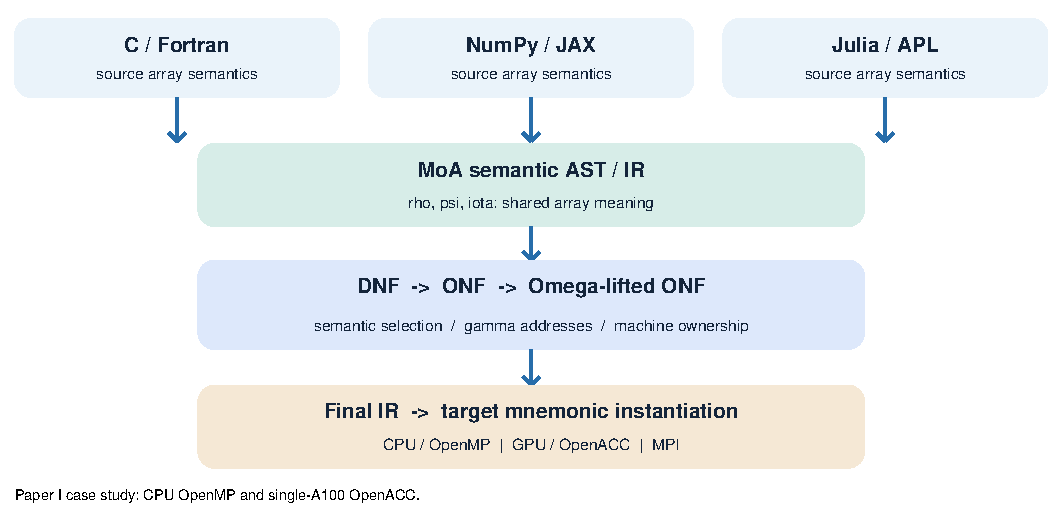
\includegraphics[width=\columnwidth]{figures/05_universal_ir_pipeline.pdf}
\Description{Pipeline from common MoA semantics through layout and machine mapping to backend realizations.}
\caption{The intended universal-IR contract: the semantic MoA AST is shared; layout, machine ownership, and backend realization vary. The diagram states the compiler architecture, not a claim that every pictured backend has been experimentally verified.}\label{fig:universal-ir}
\end{figure}

\section{From Mathematical Formulation to Predictable Execution}
The proposed compilation discipline begins with a \emph{mathematically formulated algorithm}, rather than an existing CPU or GPU loop nest. A shaped-array specification identifies the selected components and their dependencies using $\rho$, $\psi$, and $\iota$. Reduction to \emph{denotational normal form} (DNF) makes those selections explicit and provides a semantic reference independent of layout or parallelization. Reduction to \emph{operational normal form} (ONF) expresses the same selections through $\gamma$-determined addresses, $\rav$, and $[\,]$, removing unnecessary intermediates where the observable interface permits. The $\Omega$-lifted ONF then assigns components to a target machine array, subject to ownership, capacity, and communication constraints. Each stage has a different proof obligation; no stage is justified solely by an eventual speedup.

\begin{equation}\label{eq:research-chain}
\begin{aligned}
&\underbrace{\text{MoA formulation}\longrightarrow\mathrm{DNF}}_{\text{semantic selection}}
\longrightarrow\underbrace{\mathrm{ONF}_{\gamma}}_{\text{addressing}}\\
&\hspace{3em}\longrightarrow\underbrace{\Omega(\mathrm{ONF}_{\gamma},\rho M)}_{\text{machine ownership}}.
\end{aligned}
\end{equation}

The lifted ONF and a declared machine-property array are inputs to a \emph{prospective} cost calculation. A predicted mapping and performance estimate must be frozen \emph{before} running the corresponding implementation. Measured execution then validates or falsifies both the choice of mapping and the predicted time; correctness is checked independently against the original selected-component semantics. This order is essential: fitting a prediction after observing the execution cannot establish predictive power. The current Paper I evidence includes finite generated-CPU validation and preserved prospective experiments with both successes and failures, but does not establish that the full pipeline accurately predicts all CPU or GPU targets.

The motivation for this MoA-derived intermediate representation is therefore stronger than code portability alone. The same semantic DNF can admit distinct machine-dependent lifted ONFs, and the compiler can expose the chain of mathematical, resource, and performance claims for audit. The intended result is predictable performance \emph{when the cost model is validated}, not an unconditional performance guarantee.

\section{MoA Semantic Contract}
A rank-one index is written $\langle i\rangle\ps\xi$; the index is an array, not a bare scalar or an informal placeholder. For arrays $Q,K,V$ with shapes $\rho Q=\langle n,d\rangle$, $\rho K=\langle m,d\rangle$, and $\rho V=\langle m,d_v\rangle$, forward attention produces $\rho O=\langle n,d_v\rangle$. Each legal $\langle i,v\rangle\ps O$ is determined by a reduction over key index $j$ of the normalized weights associated with $\langle i,j\rangle$ and the selected value $\langle j,v\rangle\ps V$. Stable evaluation may use an online reduction summary, but its numerical contract must be stated separately from exact real-array equality.

Let $D_H$ and $D_C$ denote hand-derived and compiler-derived DNFs. Their acceptance condition is not identical derivation traces: it is equal output shape and equal selected values, $\langle i,v\rangle\ps D_H=\langle i,v\rangle\ps D_C$, for every legal index and admissible input under the declared arithmetic semantics. The archived independent interpreter exercises finite instances; it does not establish this universally.

\section{From DNF to Addressed ONF}
For a positive shape $\rho A=\langle s_0,\ldots,s_{r-1}\rangle$, consider the row-major member of the $\gamma$ layout family:
\begin{equation}
\gamma_{\rho A}(\langle i_0,\ldots,i_{r-1}\rangle)=\sum_{k=0}^{r-1}i_k\prod_{\ell=k+1}^{r-1}s_\ell.
\end{equation}
\textbf{Proposition 1 (address bijection).} On legal indices $\iota(\rho A)$, this $\gamma$ is a bijection onto $[0,\tau(A))$. Consequently $\langle i_0,\ldots,i_{r-1}\rangle\ps A=(\rav_\gamma A)[\gamma_{\rho A}(\langle i_0,\ldots,i_{r-1}\rangle)]$ for a storage realization satisfying the stated layout.

\emph{Proof sketch.} Repeated quotient--remainder decomposition recovers each index digit uniquely from the address. Conversely the mixed-radix expansion covers all addresses from zero to $\prod_k s_k-1$. This proves the mapping property, not that a particular compiler emission implements it.

\begin{figure}[t]
\centering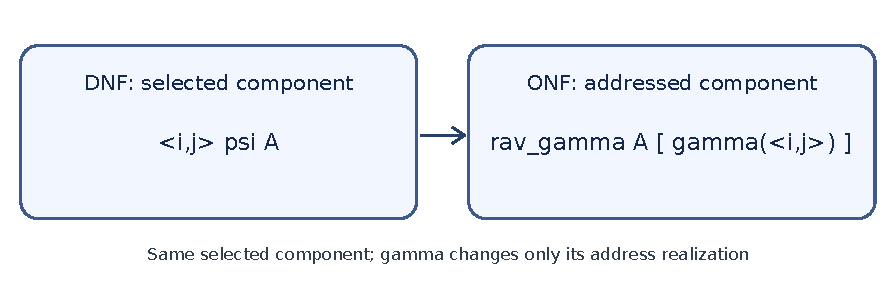
\includegraphics[width=\columnwidth]{figures/03_onf.pdf}
\Description{Legal index selection maps to a scalar address in the ravel.}
\caption{MoA index selection to addressed ONF, reproduced from the preserved master manuscript.}\label{fig:onf}
\end{figure}

\section{Machine-Dependent \texorpdfstring{$\Omega$}{Omega} Lifting}
Let the machine have shape $\rho M$ and $P=\tau(M)>0$ owner components. For $0\le q<P$ define
\begin{equation}
L_q=\lfloor qn/P\rfloor,\quad U_q=\lfloor(q+1)n/P\rfloor.
\end{equation}
The lifted ONF assigns output selections with first index $i\in[L_q,U_q)$ to owner $q$. The owner ordinal is the $\gamma$-ordered realization of an index from $\iota(\rho M)$.

\textbf{Proposition 2 (coverage and disjointness).} These half-open intervals cover $[0,n)$ exactly once, including when $P>n$; each owner writes disjoint output addresses, and the sum of assigned components is $\tau(O)=nd_v$.

\emph{Proof.} $L_0=0$, $U_{P-1}=n$, and $U_q=L_{q+1}$. Thus intervals concatenate without gaps or overlaps. Every assigned query contributes exactly $d_v$ selections. Under the selected $\gamma$, owner $q$ writes $[L_qd_v,U_qd_v)$, proving disjointness and conservation.

For $n=128$, $d_v=64$, and $\rho M=\langle2,2\rangle$, boundaries are $0,32,64,96,128$, and each owner is assigned 2048 output components. A different machine shape can produce a different lifted ONF while preserving the same semantic output.

\begin{figure}[t]
\centering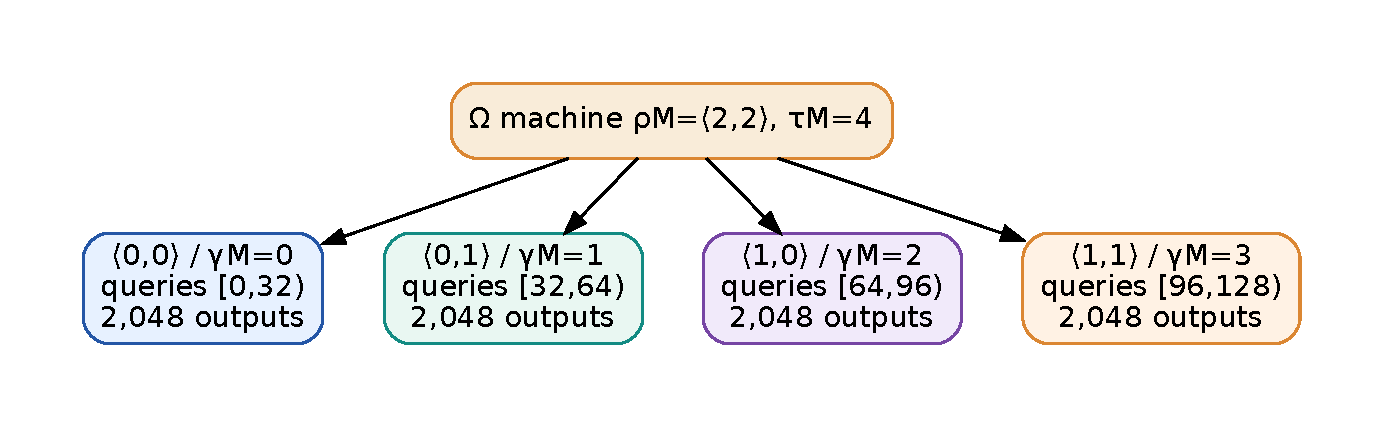
\includegraphics[width=\columnwidth]{figures/04_ownership.pdf}
\Description{Query intervals are distributed across logical owner coordinates.}
\caption{Machine-shape-dependent $\Omega$ ownership. The diagram illustrates logical ownership, not measured physical placement.}\label{fig:omega}
\end{figure}

\section{What the Compiler Produces: A Paper~I Example}
The consolidated entry point is \texttt{python moa.py attention --case p1\_forward\_cpu --out build/forward}. It exports the completed case's DNF component records, operational C AST, common-machine lift certificate and generated C. This full-output reference-schedule path is distinct from the archived O-only example below.

A useful compiler paper must show an observable output, not merely name intermediate files. Consider a typed forward-attention instance with $\rho Q=\langle3,4\rangle$, $\rho K=\langle5,4\rangle$, and $\rho V=\langle5,3\rangle$. Its output has $\rho O=\langle3,3\rangle$: nine selected scalar components, each derived from a reduction over five keys. The same selected-component DNF is the semantic reference for every legal realization. The archived Paper~I compiler accepts these extents and a logical machine shape $\rho M=\langle2,2\rangle$, then emits a C realization and a machine-ownership certificate.

\begin{figure}[t]
\centering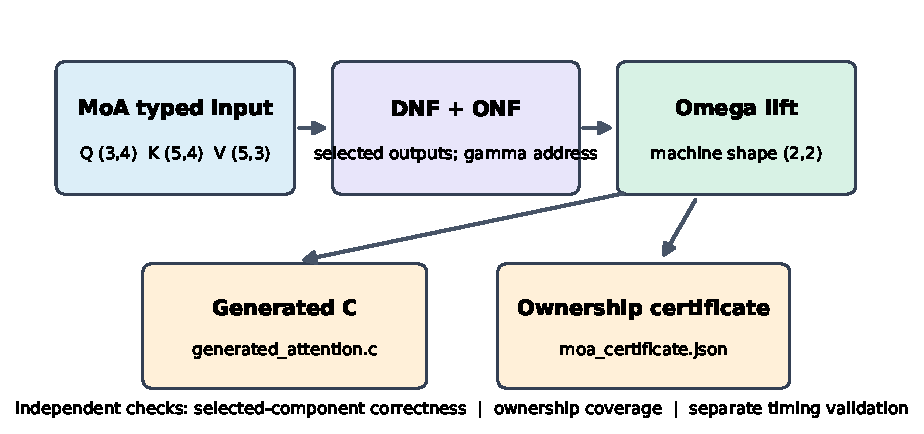
\includegraphics[width=\columnwidth]{figures/08_compiler_example.pdf}
\Description{Example input shapes, lowering stages, generated C, and ownership certificate.}
\caption{Concrete compiler output for the illustrative $\langle3,4\rangle$, $\langle5,4\rangle$, $\langle5,3\rangle$ input shapes. The emitted C and certificate are distinct artifacts: ownership coverage can be checked independently of numerical output. The displayed mapping is logical, not a physical placement guarantee.}\label{fig:compiler-example}
\end{figure}

The archived AST instance uses $n=m=128$, $d=d_v=64$, and $\rho M=\langle2,2\rangle$. The small example emits 9 output components with 4 logical owners. Their query intervals are $[0,0)$, $[0,1)$, $[1,2)$, and $[2,3)$. The executable reproduction procedure and the exact AST fields appear in Section~\ref{sec:trace-evidence}.

\section{A Worked MoA Forward-Attention Derivation}
We make the selected-component contract explicit, rather than beginning with an implementation-specific kernel. Let $Q$, $K$, and $V$ have the shapes introduced above. For legal query $i$ and key $j$, define the scalar score
\begin{equation}
 e_{ij}=\frac{1}{\sqrt d}\sum_{k=0}^{d-1}
 (\langle i,k\rangle\ps Q)(\langle j,k\rangle\ps K).
\end{equation}
Here the sum denotes a reduction of selected array components; no rank-two object is introduced to represent a vector. For each fixed $i$, define
\begin{equation}
 m_i=\max_{0\le j<m}e_{ij},\qquad
 z_i=\sum_{j=0}^{m-1}\exp(e_{ij}-m_i),
\end{equation}
\begin{equation}
 \langle i,v\rangle\ps O=\frac{1}{z_i}\sum_{j=0}^{m-1}
 \exp(e_{ij}-m_i)(\langle j,v\rangle\ps V).
 \label{eq:dnf}
\end{equation}
For nonempty key extent $m$ and finite scores, $z_i>0$. Equation~\eqref{eq:dnf} is a selected-component DNF contract. It specifies values and shapes without prescribing storage, ownership, or an execution order. The full-output interface additionally exposes the selected weights
\begin{equation}
 \langle i,j\rangle\ps A=\exp(e_{ij}-m_i)/z_i,
 \quad\rho A=\langle n,m\rangle.
\end{equation}
For the special self-attention case $n=m$ and a batch extent $B$, the weight shape is $\rho A=\langle B,N,N\rangle$, with $\rho O=\langle B,N,d_v\rangle$. The O-only path is observationally weaker: its contract cannot be used to claim that an unmaterialized $A$ has been tested.

\subsection{Hand-derived DNF versus compiler DNF: an explicit comparison}
The hand derivation of Paper~I and the frozen compiler AST use different bound-index names. Write $r$ for the key index and $h$ for the feature index. The hand-derived selected score is
\begin{equation}
 e_{ir}^{H}=d^{-1/2}\sum_{h=0}^{d-1}(\langle i,h\rangle\ps Q)(\langle r,h\rangle\ps K).
 \label{eq:handscore}
\end{equation}
The archived \texttt{01\_typed\_dnf.json} has the product \texttt{Q.indices=[i,j]}, \texttt{K.indices=[k,j]}, the score-reduction index \texttt{j}, and the key index \texttt{k}. Its mathematical reading is
\begin{equation}
 e_{ik}^{C}=d^{-1/2}\sum_{j=0}^{d-1}(\langle i,j\rangle\ps Q)(\langle k,j\rangle\ps K).
 \label{eq:compscore}
\end{equation}
The index renaming $k\mapsto r$, $j\mapsto h$ takes Eq.~\eqref{eq:compscore} \emph{exactly} to Eq.~\eqref{eq:handscore}. This establishes equality of the canonical score DNFs by comparison of the expressions. The compiler record also selects \texttt{V.indices=[k,v]}, which under the same renaming is $\langle r,v\rangle\ps V$. With the same key extent, stable maximum, exponential normalization, and weighted reduction, the selected-component output expression is therefore the hand-derived Eq.~\eqref{eq:dnf}. The independent checker distributed with this paper constructs the complete hand-output selection from Eq.~\eqref{eq:dnf}, verifies the archived compiler score and value AST selections by capture-avoiding renaming, and independently compares the materialized hand $A,O$ with an online stable $[a,z,u]$ evaluation over 160 finite cases. It checks shape and reduction bounds, not just score syntax. The JSON represents the online recurrence by a summary node and state names. The exact-real argument below establishes the mathematical equivalence of the online summary and the selected output. This archived online-summary path has a distinct contract. The later companion study closes the recovered C-emission inventory using independent exact-real component recovery and operational-tree comparisons; its scope does not certify every possible lowering of the online summary.
\begin{table}[t]
\centering\footnotesize
\caption{Visible hand/compiler DNF correspondence. Distinct derivation sequences are permitted; free indices, bounds, selections, and reduction semantics must coincide.}\label{tab:dnf-match}
\begin{tabular}{@{}p{.26\columnwidth}p{.29\columnwidth}p{.34\columnwidth}@{}}\toprule
MoA selection & Hand-derived & Compiler AST (renamed) \\\midrule
Query component & $\langle i,h\rangle\ps Q$ & $\langle i,j\rangle\ps Q$ ($j\to h$) \\
Key component & $\langle r,h\rangle\ps K$ & $\langle k,j\rangle\ps K$ ($k\to r$) \\
Score reduction & $+\red_h$ over score products & $+\red_j$ over score products \\
Value selection & $\langle r,v\rangle\ps V$ & $\langle k,v\rangle\ps V$ \\
Output & Eq.~\eqref{eq:dnf} & Stable summary $(a,z,u)$; $(\langle v\rangle\ps u)/z$ \\\bottomrule
\end{tabular}
\end{table}
\begin{figure}[t]
\centering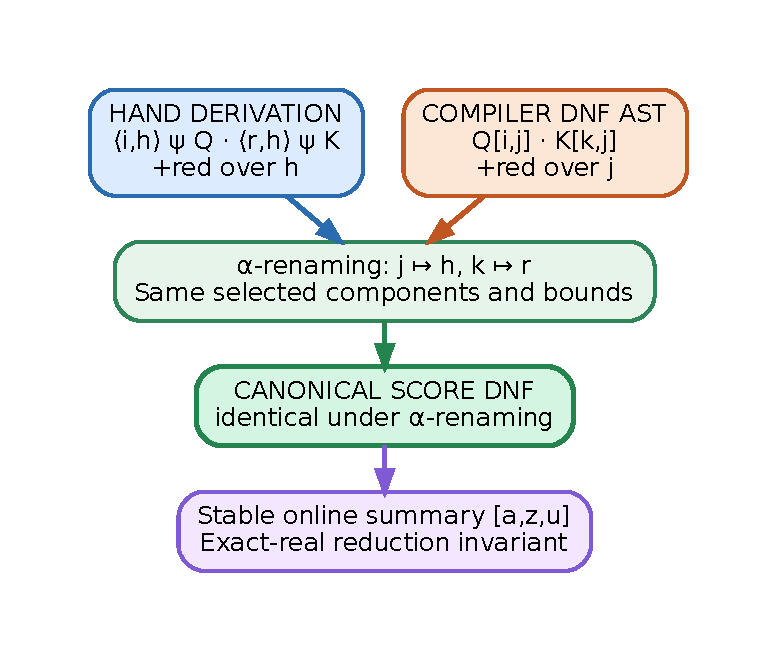
\includegraphics[width=\columnwidth]{figures/12_hand_compiler_dnf.pdf}
\Description{Hand and compiler score expressions agree after bound-index renaming.}
\caption{The evidence-bearing convergence: independent hand and compiler score expressions become identical after bound-index renaming. The next stable-summary transformation changes reduction order, not the exact-real selected-component DNF.}\label{fig:dnf-convergence}
\end{figure}

\subsection{An exact online summary under real arithmetic}
The reduction over keys can be expressed by a summary $S=(m,z,\mathbf u)$, where $m$ is the maximum score observed, $z$ is the sum of exponentials relative to $m$, and $\mathbf u$ is a rank-one array with shape $\langle d_v\rangle$. For a nonempty key subset $J$,
\begin{align}
 m_J&=\max_{j\in J}e_{ij},\\
 z_J&=\sum_{j\in J}\exp(e_{ij}-m_J),\\
 \langle v\rangle\ps\mathbf u_J&=\sum_{j\in J}\exp(e_{ij}-m_J)
 (\langle j,v\rangle\ps V).
\end{align}
For disjoint nonempty subsets $J_1,J_2$, let $m=\max(m_{J_1},m_{J_2})$ and $a_t=\exp(m_{J_t}-m)$. The combine operation is
\begin{equation}
 S_{J_1}\oplus S_{J_2}=
 (m,a_1z_{J_1}+a_2z_{J_2},a_1\mathbf u_{J_1}+a_2\mathbf u_{J_2}).
 \label{eq:combine}
\end{equation}
By substitution, the result equals $S_{J_1\cup J_2}$ componentwise. Thus $\oplus$ is associative over summaries of disjoint key subsets in exact real arithmetic. The final output selection is $(\langle v\rangle\ps\mathbf u)/z$. This algebra is the semantic reason an online fold can avoid the full intermediate. It is \emph{not} a claim of bitwise associativity for floating-point additions or exponentials.

\subsection{A finite hand-checkable example}
Take $n=3$, $m=2$, $d=2$, and $d_v=2$, so $\rho O=\langle3,2\rangle$ and $\tau(O)=6$. With $\rho M=\langle2\rangle$, the interval construction assigns query indices $[0,1)$ and $[1,3)$ to the two owners. Under the specified $\gamma$, the first owner writes output addresses $[0,2)$, and the second writes $[2,6)$. The six selections remain those of Eq.~\eqref{eq:dnf}; only their owner and address realization change. This example intentionally illustrates a nonuniform partition. It does not imply that an arbitrary machine mapping has optimal load balance.

\section{Correctness Obligations as a Commuting Diagram}
A source-to-source or source-to-machine transformation is correct only when the selected-component meanings agree along both paths. Write $\mathcal D$ for the semantic DNF, $\mathcal G_\gamma$ for address lowering, $\mathcal L_{\Omega,M}$ for ownership lifting, and $\mathcal E$ for generated execution. For admissible inputs $X$, the intended commuting condition is
\begin{equation}
 \operatorname{Obs}(\mathcal E(\mathcal L_{\Omega,M}(\mathcal G_\gamma(\mathcal D(X)))))
 =\operatorname{Obs}(\mathcal D(X)).\label{eq:commute}
\end{equation}
The observation function must identify whether the interface is O-only or full $(A,O)$. An exact equality in Eq.~\eqref{eq:commute} is a real-arithmetic statement unless a floating-point semantics and tolerance are explicitly provided.

\textbf{Lemma 1 (shape and component conservation).} A legal layout conversion preserves $\tau(A)$ and all selected-component values. For a chosen $\gamma$, address lowering changes the representation of $\langle i_0,\ldots,i_{r-1}\rangle\ps A$ into a scalar access of $\rav_\gamma A$ without changing the selection.

\emph{Justification.} The mapping is a bijection over $\iota(\rho A)$ by Proposition~1. Every legal selection is assigned one address and every address corresponds to one legal selection. Hence no component is dropped or duplicated.

\textbf{Lemma 2 (owner-independent observation).} For query-partitioned output ownership as in Proposition~2, if each owner computes its assigned selections according to the same DNF and writes only its interval, the assembled output agrees componentwise with the unlifted DNF.

\emph{Justification.} The intervals partition the legal query indices; the computation of a selected output component depends on $Q,K,V$ and its query index, not on the owner ordinal. Therefore each selected output component is computed exactly once. This does not establish correctness of shared-input transport, synchronization, or an actual implementation of the owner schedule.

\textbf{Theorem (conditional semantic preservation).} If (i) the typed DNF is equivalent to the source specification, (ii) $\gamma$ lowering implements Lemma~1, (iii) $\Omega$ lowering implements Lemma~2 and supplies all required inputs, and (iv) generated execution refines the lifted ONF under the declared arithmetic model, then Eq.~\eqref{eq:commute} holds.

\emph{Proof.} Compose the four assumed observation-preserving transformations. The conclusion is conditional on all premises; AST provenance and unit tests alone do not discharge premise (iv). This is an explicit proof-obligation decomposition, not an assertion that every premise has already been formally proved for the present compiler.

\begin{figure*}[t]
\centering
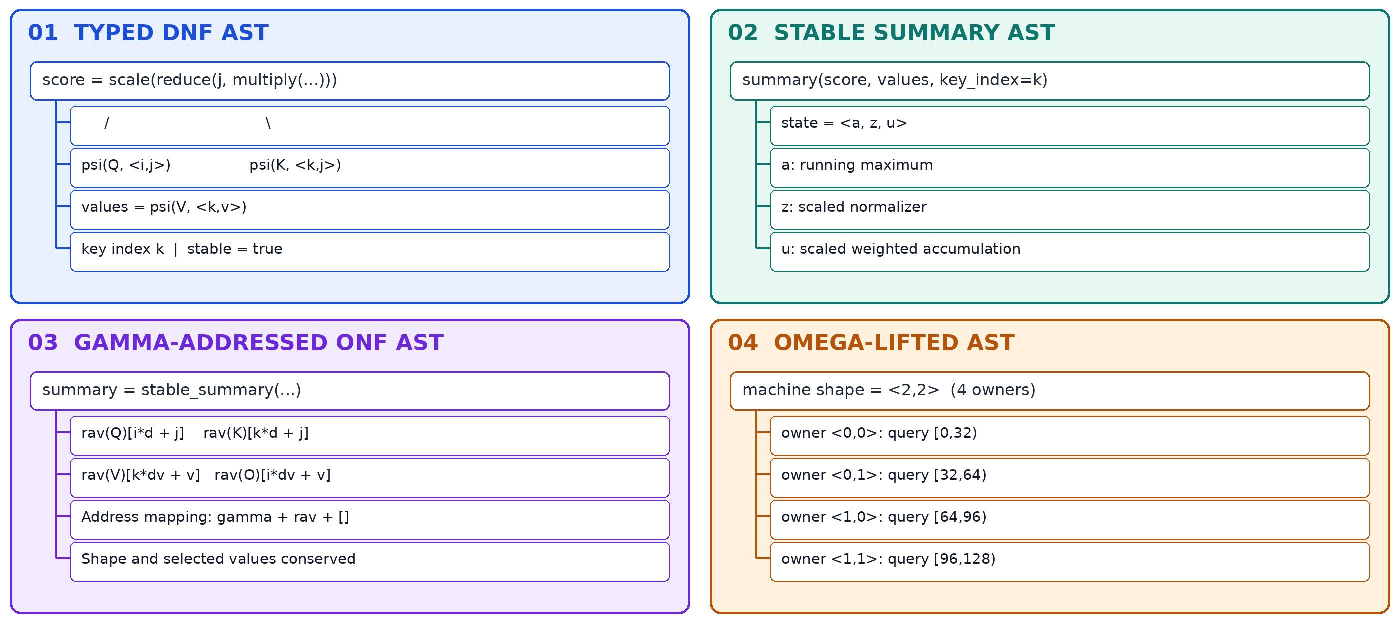
\includegraphics[width=.98\textwidth]{figures/07_typed_ast_dnf_onf_lift_READABLE.pdf}
\Description{Four panels show the typed DNF, online summary, addressed ONF, and machine owner schedule.}
\caption{Four archived Paper I AST stages for the output-only OpenMP path. Typed $\psi$ selections lead to a stable summary, $\gamma$-addressed ONF, and $\Omega$ ownership for $\rho M=\langle2,2\rangle$. The four disjoint owner intervals cover 128 queries.}\label{fig:ast-chain}
\end{figure*}

\section{Inspecting the Actual Rewrite Trace}\label{sec:trace-evidence}
The four frozen JSON records are \emph{compiler outputs}, not manually drawn replacement trees. The replay starts from a fixed typed forward-attention $\psi$ expression; its stable-fold rewrite recognizes that dependency pattern and rejects unsupported patterns. This is genuine, bounded AST rewriting, not a parser or a general-purpose $\psi$-normalization theorem. The following is a compact transcription of their checkable structure; the supplementary JSON contains every nested node. In the DNF record, \texttt{score.term.}\allowbreak\texttt{index="j"} reduces the product of the selections \texttt{Q.indices=}\allowbreak\texttt{["i","j"]} and \texttt{K.indices=}\allowbreak\texttt{["k","j"]}, with \texttt{factor="1/sqrt(d)"}; \texttt{values.indices=}\allowbreak\texttt{["k","v"]} selects $V$. The stable-summary pass introduces \texttt{state=["a","z","u"]}, representing maximum, normalization accumulator, and weighted-value accumulator. The $\gamma$ pass retains the summary and adds \texttt{addresses} for $Q,K,V$ with extents $d,d,d_v$. The $\Omega$ pass retains the addressed form and attaches owner scheduling. These fields identify the precise typed fragment exercised by the replay.

\begin{table}[t]
\centering\footnotesize
\caption{Archived compiler ASTs and their newly introduced evidence.}\label{tab:actual-asts}
\begin{tabular}{@{}p{.39\columnwidth}p{.53\columnwidth}@{}}\toprule
Frozen record & Inspectable compiler transformation \\\midrule
\texttt{01\_typed\_dnf.json} & $\langle i,j\rangle\ps Q$ and $\langle k,j\rangle\ps K$ in the score; $\langle k,v\rangle\ps V$ in the output \\
\texttt{02\_stable\_summary.json} & Stable fold state \texttt{[a,z,u]} \\
\texttt{03\_gamma\_onf.json} & Address nodes for $Q,K,V$ and widths $d,d,d_v$ \\
\texttt{04\_omega\_schedule.json} & Lowered addressed summary and machine ownership \\\bottomrule
\end{tabular}
\end{table}

\noindent\textbf{Reviewer replay.} Run \nolinkurl{bash replay.sh} from the anonymous supplement with Python 3.10 or newer. It regenerates the output-only OpenMP ASTs and C, then regenerates the measured full-output OpenACC trace and recomputes Table~\ref{tab:full-a100} from archived samples. The replay requires no GPU. Archived numerical error summaries retain the reference checks performed in the run.

\section{Compiler Pipeline and Artifact Contracts}
The typed compiler matches the supported score and value dependencies, constructs a stable summary for the output-only path, adds $\gamma$ address descriptors, and derives disjoint $\Omega$ query intervals. The full-output lowering instead uses $A$ as observable storage for scores and then weights. The following example traces the measured full-output specialization.

\paragraph{From typed contract to measured OpenACC.}
At $(B,N,D)=(2,1024,64)$ the typed DNF selects $\langle b,i,j\rangle\ps Q$, $\langle b,k,j\rangle\ps K$, and $\langle b,k,v\rangle\ps V$. Eqs.~\eqref{eq:compscore} and~\eqref{eq:dnf} apply independently at each $b$, with $A$ retained as an observable. In the materialized ONF, $A$ first holds scaled scores and is then normalized in place using a per-query maximum and sum. With $q=bN+i$, the $\gamma$ addresses for $A$ and $O$ are $qN+k$ and $qD+v$. The $\Omega$ lift assigns owner $r$ the interval $[8r,8(r+1))$ of the 2048 queries. The generated loop begins as follows.
\begin{lstlisting}[basicstyle=\ttfamily\scriptsize,columns=fullflexible,breaklines=true]
#pragma acc parallel loop gang num_gangs(256) vector_length(128)
for(size_t owner=0;owner<256;owner++){
 size_t begin=B*N*owner/256,end=B*N*(owner+1)/256;
 #pragma acc loop seq
 for(size_t q=begin;q<end;q++){
  size_t b=q/N,i=q%N;
\end{lstlisting}
The supplement regenerates the four recorded stages and complete C source byte-for-byte for this specialization. Its frozen prediction was 9.995 ms and its measured median was 9.211 ms (8.51\% error).

\subsection{What a certificate should bind}
A reproducibility certificate should bind input shapes, arithmetic assumptions, source and AST hashes, $\gamma$ layout, machine shape, owner intervals, compiler revision, emitted source hash, build flags, and independent output checks. Prospective performance evidence additionally requires a frozen prediction made before the run, its machine description, and the untouched measured results. A hash binds identity, not semantic correctness. The archived records demonstrate portions of this contract; they do not establish a complete proof-carrying compiler.

\subsection{One implementation is not every backend}
The target-language construct is an implementation choice made after MoA mapping. The demonstrated CPU OpenMP path is not automatically an OpenACC GPU or distributed MPI validation. An OpenACC source file compiled in host-fallback mode supplies CPU evidence, not GPU execution evidence. A GPU mapping additionally needs proof of ownership, memory visibility, and device-side execution for the claimed machine realization. We therefore report target-specific observations rather than collapsing them into a single generic ``portable'' result.

\section{Ten-Field Machine Description and Prediction Discipline}
The target is a shaped machine array with a canonical ten-field property record, not merely a thread count. Its indexed fields, shown in Table~\ref{tab:ten-calibration}, extend the original five-field model by five realization-sensitive properties. These are \emph{properties}, not ten spatial axes; their values may be unknown until measured, and the current Paper~I predictor does not claim to use every field.

\begin{table*}[tp]
\centering\footnotesize
\caption{Programmatic replay of predictions in \emph{One Derivation, Any Machine}. The replay takes the published calibration inputs and computes the partition before consulting the printed assignments or measurements. Rows in the last column are historical hardware evidence.}\label{tab:prediction-validation}
\begin{tabular}{@{}p{.18\textwidth}p{.25\textwidth}p{.25\textwidth}p{.25\textwidth}@{}}\toprule
Experiment & Recomputed query counts & Recomputed finish times & Historical validation \\\midrule
Two devices, $n=65{,}536$ & 47,815 / 17,721 & 24.317 / 24.317 s & 19.26 / 20.82 s \\
Three devices, $n=100{,}000$ & 89,767 / 9,511 / 722 & 531.4 / 531.5 / 531.2 ms & 358.4 / 425.0 / 2637.5 ms \\
Minimum chunk, $n=100{,}000$ & 100,000 / 0 / 0 & 592.0 ms for A100 & Actual/predicted 0.21 \\
Minimum chunk, $n=300{,}000$ & 271,261 / 28,739 / 0 & 4817.8 / 4817.8 ms & Actual/predicted 0.21 / 0.83 \\
Minimum chunk, $n=700{,}000$ & 628,370 / 66,574 / 5,056 & 26040.7 / 26040.8 / 26039.5 ms & Actual/predicted 0.23 / 0.70 / 0.72 \\
\bottomrule\end{tabular}
\end{table*}
\begin{table*}[tp]
\centering\footnotesize
\caption{Ten machine fields from \emph{Closing the Prediction Gap}. The replay uses published inputs. The validation column states the evidence required from a generated realization in a matched run.}\label{tab:ten-calibration}
\begin{tabular}{@{}p{.13\textwidth}p{.42\textwidth}p{.39\textwidth}@{}}\toprule
Field & Derivation and replay & Matched validation \\\midrule
$0:\ U_d$ & Multiply row-tile size by compute units. MI100 floor 3,840 rows. & Confirm device units and executed tiles. Hand sweep: 23 tiles before correction, 158 after. \\
$1:\ W_d$ & Group width constrains admissible tile and vector widths. & Compare actual dispatch width with requested width. \\
$2:\ M_d$ & Per-block shared-memory bound constrains tile geometry. & Compare compiler resource report and runtime occupancy. \\
$3:\ t_d$ & Hand-derived scaling: $\widehat t_d=t_dc_dn/n_0^2$ (Table~\ref{tab:prediction-validation}). & Generated A100 uses a separate affine fit per owner count. Six of eight timing predictions pass (Table~\ref{tab:full-a100}). \\
$4:\ n_d^{\max}$ & MI100 revised realization gives 33,102,053 rows from published capacity and rounded reservation. & Hand bracket $[33.1,33.3)$ million. Repeat bracket for the generated realization. \\
$5:\ M_d^{\rm cap}$ & Convert published device capacity to bytes and apply the resident-array footprint. & Device reports 81,920 MiB. Usable capacity under full-output allocation awaits bracketing. \\
$6:\ P_d$ & Use realization-specific watts. Replay yields 87.12 J for A100 at $n=100{,}000$ under fixed reference power. & Measure energy over a matched timed window and cross-check power. \\
$7:\ X_d$ & Record unit capability and bind it to live dispatch evidence. & Check specialized unit use. Hand A100 fp16 tensor active-cycle fraction was about 20.7\%. \\
$8:\ C_d$ & Pin admissible directives. A100 build logs show gang mapping and vector length 128. & NVIDIA execution probe passed. Physical occupancy and specialized-unit activity await profiling. \\
$9:\ R_d$ & Recover $1-4Dbn_{\rm pass}/M_d^{\rm cap}$ from the passing endpoint. MI100 gives 1.306\%. & Validate on an independent bracket for the selected precision and backend. \\
\bottomrule\end{tabular}
\end{table*}
The replay computes inverse-reference-time weights, selects devices whose ideal shares clear the published Intel and MI100 floors, then apportions integer query counts by largest remainder. The A100 participates in all three reported floor cases. Each device receives a contiguous interval of global queries. The replay emits OpenACC candidates with local $Q,O$ intervals and full $K,V$ extents using the same output DNF. These generated candidates use the archived FP64 emitter and have passed a compiler syntax check. Matched heterogeneous execution and calibration remain open. Replaying a ceiling with a reservation inferred from its own bracket checks arithmetic consistency. A prospective ceiling test requires an independently determined reservation.

\noindent\textbf{Machine-property coverage.} The canonical field order is $0:U_d$ compute units; $1:W_d$ group width; $2:M_d$ shared memory; $3:t_d$ reference time; $4:n_d^{\max}$ size ceiling; $5:M_d^{\mathrm{cap}}$ device capacity; $6:P_d$ power; $7:X_d$ execution-unit capability; $8:C_d$ compiler configuration; $9:R_d$ memory-reservation overhead. The recorded mapping and timing results constrain subsets of this record, \emph{not} a ten-parameter model independently calibrated end to end. In particular, compiler-generated Paper~I power and energy predictions have no validated numerical entries yet.


For a machine shape $\rho M$, the logical owner count is $P=\tau(M)$. This yields a legal mapping family, but the expression $P=\tau(M)$ alone cannot predict elapsed time. An identified physical-time model must account for the target-specific costs of reduction, memory traffic, synchronization, launch or thread overhead, and contention, under explicit measurement or calibration assumptions. Two realizations with identical logical $\rho M$ can differ in physical affinity and memory locality. The distinction is essential when interpreting an observed speedup.

A valid prospective comparison has two independently scored outcomes: whether the model selected the fastest legal candidate among those tested, and how closely its predicted time matched the measured time. A successful choice with a large absolute-time error is not an accurate timing prediction. The archived work includes both successes and failures, and the conference paper must not select only favorable cases. Any timing model refitted after observing a holdout belongs to a new, explicitly labeled experiment.

\section{Completed Hand/Compiler Correspondence Across Papers I--IV}
\label{sec:completed-suite}
The companion study independently recovers the end denotation of each structured recipe and compares it with hand equations; the emitter does not read the hand C. An independent C parser compares the emitted and hand computational regions. The complete recovered inventory contains 39 numerical routines/regions in 20 pinned C files. With Paper III's printed OpenACC listing and four explicitly derived C references, there are 44 paired cases. Original files are preserved; the four new references are not presented as archived historical C.

\begin{table}[t]\centering\footnotesize
\caption{Completed correspondence inventory; these checks add no new device timing evidence.}\label{tab:completed-suite}
\begin{tabular}{@{}lr@{}}\toprule
Check & Passing result\\\midrule
Archived numerical regions / C files & 39 / 20, all covered\\
Paired implementations & 44 / 44\\
Exact-real DNF components & 246 / 246\\
Operational/lift structures & 44 / 44\\
Untimed finite pair comparisons & 138 / 138\\
Rejected corrupted C ASTs & 109 / 109\\
Corrected fresh-device entry pairs & 5 / 5\\\bottomrule
\end{tabular}\end{table}

The covered backward components include the selected gradients $GQ,GK,GV$; decode covers GQA/MQA/MHA head sharing and cache append including an empty cache; the block components cover RMS normalization, gated FFN and composed forward/backward roots. All 246 independently recovered component comparisons pass. Different schedules may have different ONFs: equality is required \emph{within each chosen hand/compiler pair}, not between all attention algorithms. Five matched entry corrections transfer host-zeroed additive accumulators to fresh device storage; the original archived variants remain available.

The C comparison preserves types, scalar arithmetic order, loop bounds, allocation positions, atomics, helpers and parallel/data directives. Normalization removes formatting and compares integer address polynomials under no-overflow premises; it does not reassociate floating-point reductions. Equal operational trees yield equal lifted trees only under the same admissible machine shape, binding, workspace, reduction tree and runtime choices. The ownership/tile/head checks include 259, 280 and 119 finite cases, respectively. This is trusted executable translation validation, not a universal compiler-correctness theorem.

A consolidated release exports the existing certificate and explicit DNF, ONF and lifted-ONF records for each case. It first checks that the current recipe and addressed AST match their completed proof identities. Integration replay verifies those identities without restarting the derivation study. The bounded Fortran extension and its host tests remain a separate scope.

The Paper V hand measurements provide empirical context. Matching denotations and addressed structures support transferring mathematical work and logical-access analysis, but unconditional timing transfer also requires the exact executed source/build, machine, mapping, workload, precision, outputs and timing boundary. Some historical source/build bindings remain absent. No new timing experiment is needed to establish the correspondence equalities; later experiments test new machine/runtime or performance claims.

\section{Independent Validation Protocol}
\subsection{Numerical comparison}
For a finite test input, the reference and generated outputs should be constructed independently and compared for every legal output index. A reported maximum absolute error $\epsilon_\infty$ means
\begin{equation}
 \epsilon_\infty=\max_{\langle i,v\rangle\in\iota(\rho O)}
 \left| (\langle i,v\rangle\ps O_{\mathrm{generated}})-
 (\langle i,v\rangle\ps O_{\mathrm{reference}})\right|.
\end{equation}
This finite statistic is meaningful only with the input shapes, values, reference implementation, and floating-point conditions attached. Tests should include nondivisible owner counts, singleton key extents, unequal key/query extents, and multiple batch instances where the interface supports batching. A full-output test must independently compare both $A$ and $O$, not merely verify the latter.

\subsection{Experimental identity and failure handling}
The evidence archives must distinguish the hand-derived historical programs from compiler-generated programs and keep exact source identity with the reported timings. The verified November 10 historical audit found 11 source/data files byte-identical to the nested software archive and checked 64 CPU rows and 16 corrected GPU rows. These checks support provenance for the retained files; they do not make every historical timing independently reproducible. The full-output OpenACC campaign supplies new device evidence for the generated realization in Table~\ref{tab:full-a100}.

\section{Attention-Compiler Comparison and Falsifiable Novelty}
\label{sec:fair-comparison}
Our relevant comparison is with \emph{AI attention compilation}, not unrelated compiler workloads. Online normalization~\cite{online} supplies the stable maximum and normalizer update. FlashAttention~\cite{flash,flash2} supplies IO-aware exact-attention algorithms and stable blockwise execution; Triton~\cite{triton} exposes GPU tile-level programming; TVM~\cite{tvm} supports hardware-aware generation and schedule selection. PyTorch attention provides a widely used execution baseline. MoA's distinct question is whether a canonical $\psi$-DNF, $\gamma$-addressed ONF, and machine-shaped $\Omega$ mapping can be derived and audited together, with a prospectively frozen resource/time prediction. We do not claim speedup over any of these systems without matched attention contracts and hardware measurements.

Lift~\cite{lift} uses functional parallel patterns and rewrite rules to express GPU mappings. In this case study, MoA makes three boundaries directly inspectable: the typed $\psi$ DNF records selections and reduction domains for comparison with the hand derivation, $\gamma$ records the address of each operand selection, and $\Omega$ records query ownership for the chosen machine shape. The emitted source and frozen holdout records connect those passes to the measured realization. The prospective hardware evidence remains specific to Paper I; the companion correspondence scope additionally covers the recovered C implementations in Papers II--IV.

\section{Evidence of Automated MoA and Machine Properties}
\label{sec:evidence-matrix}
The evidence chain is: frozen typed $\psi$-DNF $\rightarrow$ stable reduction AST $\rightarrow$ addressed $\gamma$-ONF $\rightarrow$ $\Omega$ owner schedule $\rightarrow$ generated C $\rightarrow$ independent finite execution checks. Table~\ref{tab:actual-asts} identifies the preserved intermediate records, while Tables~\ref{tab:prediction-validation} and~\ref{tab:ten-calibration} connect the historical predictions and measured machine properties to the current compiler validation boundary. Machine properties are not ten machine dimensions and are not all calibrated by the current compiler.

\begin{figure}[t]
\centering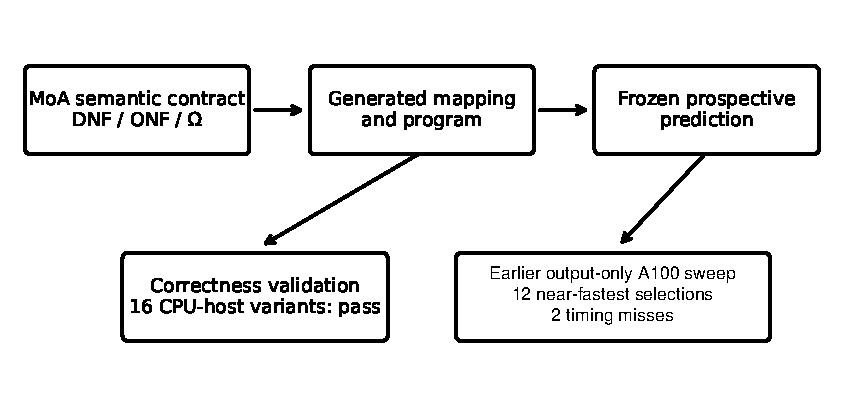
\includegraphics[width=\columnwidth]{figures/06_validation_story.pdf}
\Description{Evidence connects the mathematical stages with generated execution and prediction validation.}
\caption{Separate, inspectable evidence obligations: MoA semantics, legal $\gamma/\Omega$ mapping, executable realization, and observed behavior.}\label{fig:validation-story}
\end{figure}

\paragraph{Generated execution.}
The archived OpenMP CPU run measured 2.620910 ms at one thread and 0.658304 ms at four threads ($3.981309\times$), with maximum output error $9.99\times10^{-16}$. The earlier output-only OpenACC campaign is a separate observable contract. Here the generated full-output lowering materializes scores in $A$, normalizes each row in place, and produces $O$. Its archived stages record the $\psi$ dependencies, stable materialized ONF, $\gamma$ addresses, and $\Omega$ intervals over $BN$ queries.

\paragraph{Prospective full-output A100 validation.}
On one A100-SXM4-80GB, $B=2$, $D=64$, $\rho A=\langle B,N,N\rangle$ and $\rho O=\langle B,N,D\rangle$. The historical GPU input generator uses 32-bit unsigned state. Array storage and kernel arithmetic are FP64. We calibrated a nonnegative affine timing law in $BN^2D$ for each candidate at $N=96,384,1536$, then froze predictions for the eight sizes in Table~\ref{tab:full-a100}. The timed boundary is one synchronous generated call including transfers of inputs and both outputs, with host allocation and input generation outside the timer. Each size and candidate has seven timed samples after warmup. NVIDIA device probes passed for all 32 combinations. An independently materialized NumPy reference computes scaled scores, max-shifted normalization, and the weighted output. The run checks each returned component of both arrays for finiteness and agreement with absolute and relative tolerances of $10^{-12}$.

The audit verified 401 frozen files and the runner and compiler hashes. Recomputing medians from 224 samples gave the results below. The largest archived absolute errors versus the run's independent reference were $2.78\times10^{-17}$ for $A$ and $2.26\times10^{-16}$ for $O$. The archived error summaries and output digests support inspection of the reported checks. Independent error recomputation requires the output arrays or fresh execution.

\begin{table}[t]
\centering\footnotesize
\caption{Full-output A100 holdout. The predicted owner count is 256 for every size. Time is in milliseconds for that candidate. Error is absolute relative error against its observed median.}\label{tab:full-a100}
\begin{tabular}{@{}rrrrr@{}}\toprule
$N$ & Median winner & Predicted & Median & Error (\%)\\\midrule
64 & 128 & 0.271 & 0.172 & 57.75 \\
128 & 256 & 0.386 & 0.299 & 28.88 \\
256 & 256 & 0.843 & 0.858 & 1.75 \\
512 & 256 & 2.674 & 2.677 & 0.11 \\
1024 & 256 & 9.995 & 9.211 & 8.51 \\
2048 & 256 & 39.282 & 43.659 & 10.02 \\
4096 & 256 & 156.428 & 145.943 & 7.18 \\
8192 & 256 & 625.013 & 684.407 & 8.68 \\
\bottomrule
\end{tabular}
\end{table}

Selection regret was below 1.05 at every size. At $N=64$, $\Omega\langle128\rangle$ had the lowest observed median (0.171415 ms), while $\Omega\langle256\rangle$ had a 0.345\% higher median (0.172006 ms). Their seven-sample timing ranges overlapped. A fixed $\Omega\langle256\rangle$ rule makes the same choices. Timing predictions passed the 25\% threshold at six sizes, with overpredictions at $N=64$ and $128$. The first CPU holdout missed the fastest shape by a factor of 3.95 in observed time. The second chose the fastest tested shape with predicted time 26.80 times its measured median. A matched PyTorch baseline was unavailable on the A100 run.

\section{Related Work and Conclusion}
The comparison is restricted to AI attention implementations and compilers: FlashAttention~\cite{flash,flash2}, Triton~\cite{triton}, and TVM~\cite{tvm}, with PyTorch attention as a practical reference. Our distinct, falsifiable contribution is an auditable MoA selected-component contract through addressing, machine-shape lifting, and prospective prediction; matched performance superiority is not established.

This Paper~I compiler case study establishes a positive, executable foundation for mechanizing hand-derived MoA: inspectable $\psi$ reductions, $\gamma$ addressing, $\Omega$ mapping, and validated CPU OpenMP execution and a full-output OpenACC holdout on one A100. The companion study additionally closes all 44 declared hand/compiler C pairs across Papers I--IV, with 246 matching exact-real DNF components and matching operational/common-machine lifted structures. These correspondence results remain distinct from the target-specific prediction evidence. Completing the ten-field machine model requires independent capacity, power, energy, and dispatch measurements for the generated realization~\cite{prediction,oneDerivation}.

\section{Future Research}
Hand/compiler correspondence for the recovered C implementations in Papers I--IV is completed within Section~\ref{sec:completed-suite}'s contracts. Future work extends this foundation rather than repeats it: a shared typed cross-family IR, broader array-language frontends, additional admissible target mappings, and independent capacity/power/energy/dispatch validation for generated realizations. Paper V~\cite{hardware} remains the empirical reference; missing executed-source/build identities must be recovered before unconditional quantitative timing transfer. AI algorithms are the initial domain for mathematically formulated, portable, scalable, predictable and validated array designs. New targets and cost laws require their own frozen predictions and independent evidence.


\begin{thebibliography}{25}
\bibitem{moa} Lenore M. Mullin. 1988. \emph{A Mathematics of Arrays}. Doctoral dissertation.
\bibitem{online} Maxim Milakov and Natalia Gimelshein. 2018. Online Normalizer Calculation for Softmax. arXiv:1805.02867. \url{https://arxiv.org/abs/1805.02867}.
\bibitem{paperI} Lenore M. Mullin and Gaëtan Hains. 2026. Attention at the Theoretical Minimum: A Mathematics of Arrays Framework for Memory-Optimal Transformer Kernels. arXiv:2606.07713. \url{https://arxiv.org/abs/2606.07713}.
\bibitem{paperII} Lenore M. Mullin and Gaëtan Hains. 2026. Attention at the Theoretical Minimum: Backward Pass MoA DNF Derivation, PyTorch Implementation, and Numerical Verification. HAL:hal-05659212. \url{https://hal.science/hal-05659212}.
\bibitem{paperIII} Lenore M. Mullin and Gaëtan Hains. 2026. MoA decode attention with KV cache and grouped/multi-query attention (hand-derived). arXiv:2607.19456. \url{https://arxiv.org/abs/2607.19456}.
\bibitem{paperIV} Lenore M. Mullin and Gaëtan Hains. 2026. MoA Transformer block including RMSNorm and feed-forward layers (hand-derived). HAL:hal-05734881. \url{https://hal.science/hal-05734881}.
\bibitem{hardware} Lenore M. Mullin and Gaëtan Hains. 2026. Validating Memory-Optimal Transformer Kernels on Real Hardware: From Formal Derivation to Measured Performance Across Two HPC Clusters. arXiv:2609.33916. \url{https://arxiv.org/abs/2609.33916}.
\bibitem{oneDerivation} Lenore M. Mullin and Gaëtan Hains. 2026. One Derivation, Any Machine. Research manuscript.
\bibitem{prediction} Lenore M. Mullin and Gaëtan Hains. 2026. Closing the Prediction Gap: Completing Machine Shape So That Predicted Time, Power, Energy, and Mapping Match What Real Hardware Does. arXiv:2610.03197. \url{https://arxiv.org/abs/2610.03197}.
\bibitem{tvm} Tianqi Chen, Thierry Moreau, Ziheng Jiang, Lianmin Zheng, Eddie Yan, Haichen Shen, Meghan Cowan, Leyuan Wang, Yuwei Hu, Luis Ceze, Carlos Guestrin, and Arvind Krishnamurthy. 2018. TVM: An automated end-to-end optimizing compiler for deep learning. \emph{OSDI}, 578--594.
\bibitem{flash} Tri Dao, Daniel Y. Fu, Stefano Ermon, Atri Rudra, and Christopher R\'e. 2022. FlashAttention: Fast and memory-efficient exact attention with IO-awareness. \emph{NeurIPS} 35, 16344--16359.

\bibitem{flash2} Tri Dao. 2024. FlashAttention-2: Faster Attention with Better Parallelism and Work Partitioning. \emph{ICLR}. \url{https://proceedings.iclr.cc/paper_files/paper/2024/hash/98ed250b203d1ac6b24bbcf263e3d4a7-Abstract-Conference.html}.

\bibitem{triton} Philippe Tillet, H. T. Kung, and David Cox. 2019. Triton: An Intermediate Language and Compiler for Tiled Neural Network Computations. \emph{MAPL}, 10--19. DOI: 10.1145/3315508.3329973.

\bibitem{lift} Michel Steuwer, Toomas Remmelg, and Christophe Dubach. 2017. Lift: A Functional Data-Parallel IR for High-Performance GPU Code Generation. \emph{CGO}, 74--85.
\end{thebibliography}


\end{document}
